%%
%% Capítulo 2: Expressões matemáticas
%%

\mychapter{Trabalhos relacionados}
\label{Cap:TrabalhosRelacionados}


\section{MuZero}

MuZero é um sistema de máquina que utiliza algoritmos de
aprendizado por reforço e aprendizado supervisionado para
resolver jogos de atari, xadrez e Shogi também conhecido como
xadrez japonês, o MuZero é um sistema com três componentes:
Representação, dinâmica e predição, Representação é uma uma
função $h_{\theta}$  que recebe $t$ observações 
e cria uma Representação interna $s$, $s = h_{\theta}(o_1,...,o_t)$,
onde $o$ é uma observação, uma observação pode ser entendia como sendo
um vetor que contem todos os valores dos sensores em um instante $t$.
A predição é uma função $f_{\theta}$ que recebe uma representação $s$
e retorna uma vetor de valores $v[k]$ que dizem o quão boa seria tomar
uma decisão discreta $k$,  $v[k] =  f_{\theta}(s)$ ,
para cada ação discreta $k$, uma ação $a$,poderia ser o índice do maior
valor de $v^{k}$ ou utilizar a busca em árvore do Monte Carlo através do
modelo de dinâmica, o modelo de dinâmica é uma outra função
$g_{\theta}$, que busca prever dado uma ação $a^k$ e um estado $s^{k}$,
encontra o estado $s^{k+1}$ e sua recompensa $r^{k+1}$ associado ao estado,
ou seja, $s^{k+1},r^{k+1}=  g_{\theta}(s^{k},a^k)$.


\begin{figure}[H]
    \centering
    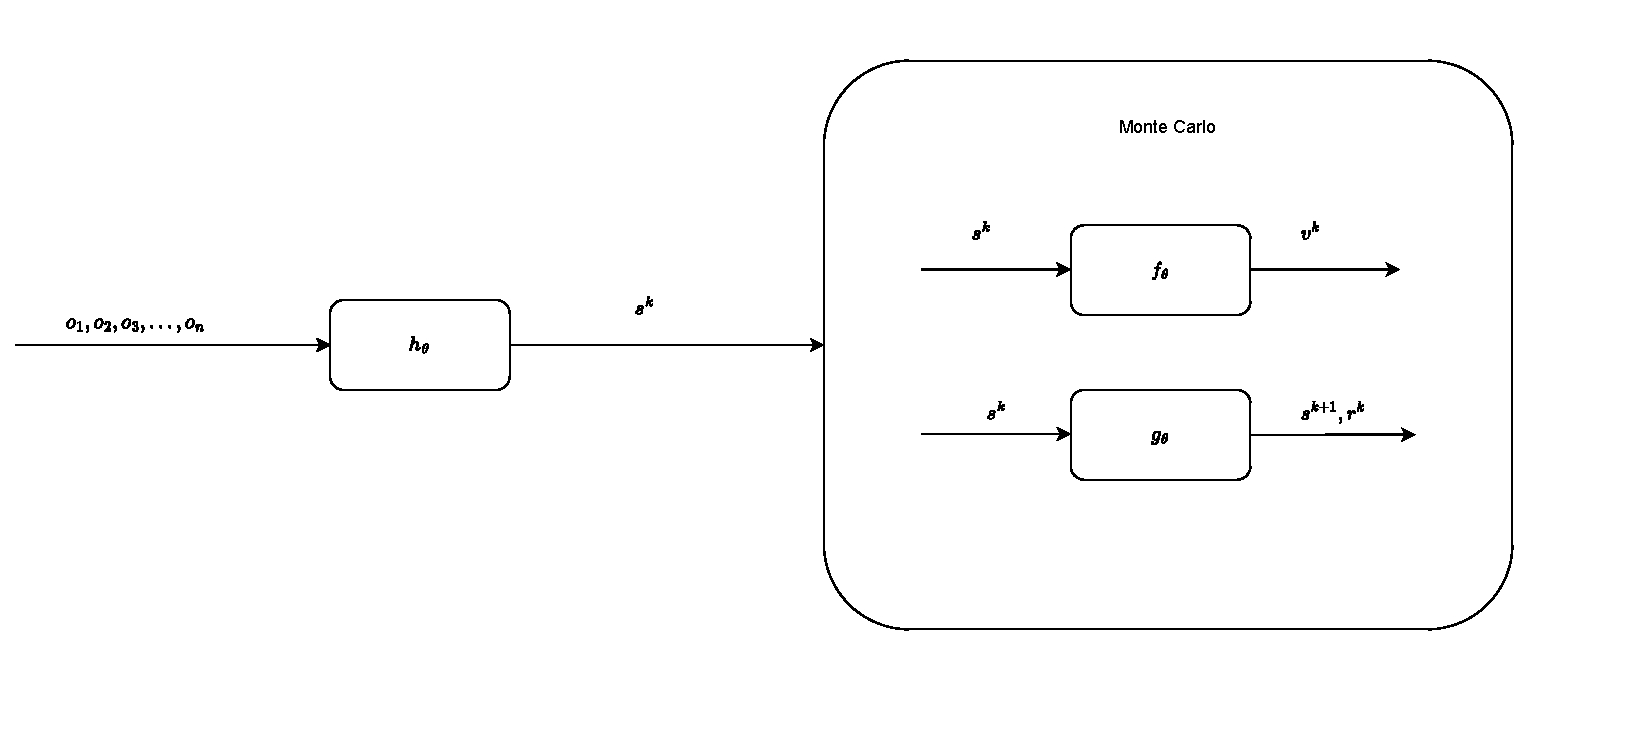
\includegraphics[scale=0.4]{figuras/muzero_dig.pdf}
    \caption{diagrama dos modelos do Muzero}
\end{figure}

A importância do MuZero para este trabalho não se trata do modelo em si,
mas sim a forma como resolveu o problema, dividindo o sistema em componentes
de forma muito semelhante  em teoria de controle, onde
o modelo de predição  $f_{\theta}$ pode ser entendido algo
análogo ao controlador,o  modelo dinâmico $g_{\theta}$ como a planta,
e $h_{\theta}$ sendo os sensores, sendo $h_{\theta}$ o modelo
necessário  para que o sistema seja genérico o suficiente para jogar
diferentes jogos. É importante destacar a diferença entre o controlador P.I.D
toma decisões a partir de instantes $t_n,t_{n-1},...t_{0}$, já o $f_{\theta}$
com a buscar Monte Carlo toma decisões em $k$ instantes futuros utilizando
a função $g_{\theta}$ análoga a planta.

\begin{figure}[H]
    \centering
    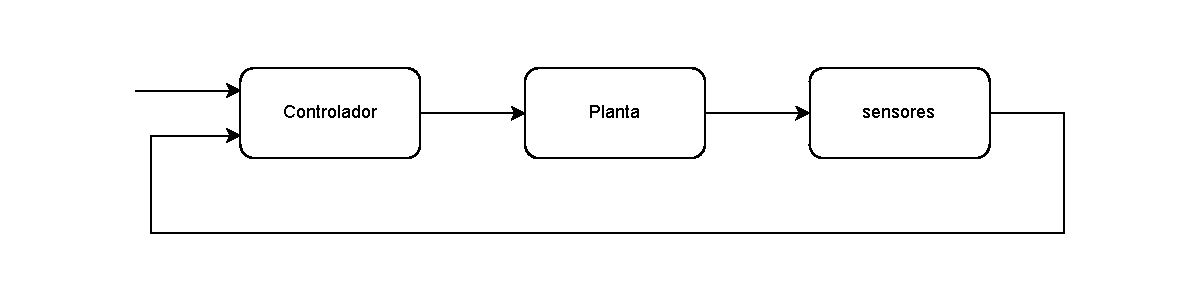
\includegraphics[scale=0.6]{figuras/sistema_classico_controle.pdf}
    \caption{diagrama clássico de controle}
\end{figure}

\section{Controlador de posição e aprendizado por reforço }

Utilização de aprendizado por reforço para criação de controladores
de retroalimentação, foi observado em \cite{farias2020position}
a qual mostrou que o algoritmo \textit{Q-learning} é capaz de aprender
as regras de um controlador com estrições de velocidades linear e angular
para  posicionar o robô em determinada posição, no entanto em seus
experimentos foram necessários 5 milhões de iterações para se ter um modelo
inferior a um controlador que utiliza as leis clássicas de controle.

\subsection{Q-learning}
\textit{Q-learning} é um algoritmo de aprendizado por reforço que
busca aprender uma função ação-valor $Q$ que diretamente aproxima
a função ação-valor ótima $Q^*$ independe do algoritmo utilizado
para selecionar uma ação. \textit{Q-learning} é definido:

\begin{equation} 
    Q(S_t,A_t) \leftarrow Q(S_t,A_t) + \alpha[R + \gamma  \max_aQ(S_{t +1},a) - Q(S_t,A_t)]
\end{equation}
onde $S_t$ e $A_t$ é respectivamente estado,ação,  $ \max_a Q(S_{t +1},a)$ é o valor da
ação de maior valor no estado $S_{t+1}$ e as constantes $\alpha$, $\gamma$ são taxas
de aprendizado que variam de 0 até 1. É muito comum representar a função $Q$
sendo uma tabela, onde o estado $S$ e ação $A$ são indices, e em contexto de
controladores de retroalimentação para robôs moveis, o estado pode ser um
valor de distância até o alvo discretizado e ação pode ser movimentos simples
como girar para esquerda,direita, ir para frente e rê. Por fim o valor é
número continuo ou discreto derivado de uma função recompensa que poder
a a variação de distância até o alvo observada após o movimento. O algoritmo
Q-learning é apresentado em Algoritmo  \ref{Q-learning:}


\begin{algorithm}[H]
    \label{Q-learning:}
    Parâmetros dos algoritmo: importância de um paço $\alpha \in (0,1]$
    taxa de aprendizado $\gamma \in (0,1] $

    
    \Entrada{$N_e$:número de epsodios; $N_p$ = número de paços}
    %% \SetLine
    
    inicialize $Q(s,a)$ arbitrariamente exceto $Q(\text{terminal},\cdot ) = 0$

    \Para {$e \leftarrow 0$ \Ate $N_e$} {
        inicialize o $S$ com o estado inicial $S_0$

        
        \Para {$j \leftarrow 0$ \Ate $N_p$} {
            Escolha a ação $A$ do estado $S$ usando alguma regra derivada de $Q$,
            por exemplo a $\epsilon$-greedy

            Realize a ação $A$ e observe a recompensa $R$ e o novo estado $S'$
            
            $Q(S,A) \leftarrow (S,A) + \alpha[R + \gamma \max_aQ(S',a) - Q(S,A)]$
            
            $S \leftarrow S'$


            \Se {S é terminal}{
                
              $j \leftarrow N_p$  \textbf{ fim do loop de paços}
            }
        }
        
    }
    \Retorna $Q(s,a)$
    \caption{Algoritmo Q-learning}
    
\end{algorithm}

Em \cite{quiroga2022position}
foram utilizado algoritmos variantes do \textit{Q-learning}, como \textit{Deep Q-learning Network} e \textit{Deep Deterministic Policy Gradient},
para encontrar as regras de um controlador que posicione o robô em determinada
posição e evite de obstáculos usando sensores ultrassônicos, apesar do sucesso
os algoritmos não enviam os sinais de velocidades angulares
diretamente para o modelo cinemático do robô, os sinais
eram a entrada do algoritmo de Braitenberg, um algoritmo que converte
sinais de distância de obstáculos em velocidades lineares e angulares
que evitam a colisão com obstáculos, além do treinamento permitir que o robô
colida com um obstáculo foi observado que o tempo de treinamento desses modelos
foram de 8,6 e 11,4 horas de treinamento para \textit{Deep Q-learning Network}
e \textit{Deep Deterministic Policy Gradient}, respectivamente, segundo o
artigo o melhor o controlador foi o \textit{Deep Deterministic Policy Gradient}
que conseguiu chegar na posição desejada 3 segundos mais rápido do que o
melhor controlador que utiliza as leis clássicas de controle isso em um ambiente sem
obstáculos e em um ambiente com obstáculos a diferença aumentou para
17,3 segundos, no entanto a distância do robô até os obstáculos ficou
inferior a 20 centímetros, ou seja, o modelo de aprendizado encurtou o
caminho ficando mais próximo de bater no obstáculo, é importante dizer que
em ambos os trabalhos utilizaram um robô de acionamento diferencial.

\subsection{Deep Q-learning e Deep Deterministic Policy Gradient }
\textit{Deep Q-learning Network} é o algoritmo \textit{Q-learning}
aplicado a redes neurais de modo que a função gerada pelo treinamento
dessa rede é uma aproximação da função valor ótima $Q^*$, uma das vantagens
de utilizar redes neurais é fato de poder utilizar estados continuos sem a
necessidade de discretização, no entanto o espaço de ação ainda é necessário
ser discreto. Muitas das vezes esse algoritmo é utilizado
tendo como estado $S$ sendo uma imagem que normalmente é preprocessada
antes de enviada para a rede neural. Para ter um treinamento mais estável,
se é utilizado duas redes, onde a rede alvo é atualizada usando o parâmetro
de polyak $\rho$ após o fim de uma época $e$.
O algoritmo do \textit{Deep Q-learning Network}
pode ser vista no Algoritmo \ref{Deep:Q-learning:}

\begin{algorithm}[H]
    %% \SetLine
    Parâmetros dos algoritmo:
    importância de um paço $\alpha \in (0,1]$,
    taxa de aprendizado $\gamma \in (0,1]$,
    polyak $\rho \in (0,1]$,
    capacidade da memória $C \in \mathbb{N}$ 


    inicialize os pesos $\theta$ da rede neural que aproxima a função $Q$ com valores aleatórios

    inicialize os pesos $\theta_{\text{target}}  \leftarrow \theta$ rede alvo $Q_{\text{target}}$

    \Para {$e \leftarrow 0$ \Ate $E$} {
        inicialize a sequencia $s_0$

        inicialize a sequência preprocessada $\phi_0 \leftarrow \phi(s_0)$ 
        

        \Para {$j \leftarrow 0$ \Ate $n$} {
            Escolha a ação $a_t$ do estado processado $phi_t$ usando alguma regra derivada de $Q$,
            por exemplo a $\epsilon$-greedy

            Realize a ação $a_t$ e observe a recompensa $r_t$ e o nova imagem $x_{t+1}$
            
            $s_{t+1}  \leftarrow (s_t, a_t, x_{t+1})$   

            preprocesse a sequencia $\phi_{t+1} \leftarrow \phi(t+1)$
            
            armazene a transição $(\phi_t,a_t,r_t,\phi(t+1))$ na memória $M$

            \Se {$K \ge$ total de transições armazenadas}{
                Selecione $K$ amostras para formar um minibatch de transições

                inicialize o conjunto $y$ de valores desejados
    
                \Para {$k \leftarrow =0$ \Ate $K$}{
    
    
                    \eSe {$s_k$ é terminal}{
                    
                        $y_k \leftarrow r_k$
                      }
                      {
                        $y_k \leftarrow r_k + \gamma \max_aQ(\phi_k,a_k)$
                      }
                    
                }
    
                atualize os pesos $\theta$ baseado no erro $\frac{1}{|K|} \sum_{b =0}^{K}(y -Q(\phi_b,a_b))^2$

        
            }

            \Se {$s_{t+1}$ é terminal}{
                
                $j \leftarrow N_p$  \textbf{ fim do loop de paços}
              }

        }

        ao fim de uma época,atualize os pesos da rede alvo
        $\theta_{\text{target}}  \leftarrow \rho \theta_{\text{target}}  + (1-\rho) \theta$
        
    }
    \Retorna a rede neural $Q_{\text{target}}$
    \caption{Algoritmo Deep Q-learning}
    \label{Deep:Q-learning:}
\end{algorithm}

Como dito anteriormente A \textit{Deep Q-learning}, possuí o espaço das ações são discretas,
visando tornar o espaço de ações também continuas é acrescentando mais
uma rede neural para aproximar a política $\mu$,
desta forma temos um algoritmo baseado na equação \textit{Q-learning} que permite
aprender um sistema de entrada e saída contínua.
\begin{flalign} 
    A_t = \mu(S_t)\\
    Q(S_t,A_t) \leftarrow Q(S_t,A_t) + \alpha[R + \gamma  Q(S_{t +1},\mu(S_{t+1})) - Q(S_t,A_t)]
\end{flalign}
Enquanto temos uma rede neural $Q$ que busca encontrar a função ação-valor ótima $Q^*$, temos uma
nova rede neural que através do gradiente ascendente buscar encontrar a política $\mu$
que maximiza a recompensa da função valor aproximada $Q(S,\mu(S))$. O algoritmo do \textit{Deep Deterministic Policy Gradient}
pode ser vista no Algoritmo \ref{Deep Deterministic Policy Gradient:}

\begin{algorithm}[H]
    %% \SetLine
    Parâmetros dos algoritmo:
    importância de um paço $\alpha \in (0,1]$,
    taxa de aprendizado $\gamma \in (0,1]$,
    polyak $\rho \in (0,1]$,
    capacidade da memória $C \in \mathbb{N}$ 

    inicialize a memória $M$ com a capacidade $C$

    inicialize os pesos $\theta$ da rede neural que aproxima a função $Q$ com valores aleatórios

    inicialize os pesos $\theta_\mu$ da rede neural que a aproxima da política $\mu(\phi)$ com valores aleatórios

    inicialize os pesos $\theta_{\text{target}}  \leftarrow \theta$ rede alvo $Q_{\text{target}}$

    inicialize os pesos $\theta_{\mu_{\text{target}}}  \leftarrow \theta_\mu$ rede alvo $\mu_{\text{target}}$


    \Para {$e \leftarrow 0$ \Ate $E$} {
        inicialize a sequencia $s_0$

        inicialize a sequência preprocessada $\phi_0 \leftarrow \phi(s_0)$ 
        

        \Para {$j \leftarrow 0$ \Ate $n$} {
            Escolha a ação $a_t$ do estado processado $phi_t$ usando a rede  $\mu(\phi) + \epsilon$, onde
            $\epsilon$ é um ruído que controla a exploração, $a_t \leftarrow \mu(\phi_t)  + \epsilon$ 

            Realize a ação $a_t$ e observe a recompensa $r_t$ e o nova imagem $x_{t+1}$
            
            $s_{t+1}  \leftarrow (s_t, a_t, x_{t+1})$   

            preprocesse a sequencia $\phi_{t+1} \leftarrow \phi(t+1)$
            
            armazene a transição $(\phi_t,a_t,r_t,\phi(t+1))$ na memória $M$

            \Se {$K \ge$ total de transições armazenadas}{
                Selecione $K$ amostras para formar um minibatch de transições

                inicialize o conjunto $y$ de valores desejados
    
                \Para {$k \leftarrow =0$ \Ate $K$}{
    
    
                    \eSe {$s_k$ é terminal}{
                    
                        $y_k \leftarrow r_k$
                      }
                      {
                        $a_d = \mu_{\text{target}}(\phi_k)$
    
                        $y_k \leftarrow r_k + \gamma Q_{\text{target}}(\phi_k,a_d)$
                      }
                    
                }

                atualize os pesos $\theta$ baseado no erro  $\frac{1}{|K|} \sum_{b =0}^{K} (y -Q(\phi_b,\mu(\phi_b)))^2$
                
                atualize os pesos $\theta_\mu$ baseado no gradiente ascendente:
                $\nabla_{\theta_\mu} \frac{1}{|K|} \sum_{b =0}^{K} Q(\phi_b,\mu(\phi_b))$
            
            }

           
        }

        atualize os pesos da rede alvo $\theta_{\text{target}}  \leftarrow \rho \theta_{\text{target}}  + (1-\rho) \theta$

        atualize os pesos da rede alvo $\theta_{\mu_{\text{target}}}  \leftarrow \rho \theta_{\mu_{\text{target}}}  + (1-\rho)\theta_\mu$

        
    }
    \Retorna as redes neurais $Q_{\text{target}}$, $\mu_{\text{target}}$
    \caption{Algoritmo Deep Deterministic Policy Gradient}
    \label{Deep Deterministic Policy Gradient:}
\end{algorithm}


\subsection{Conclusão da revisão bibliográfica}
Os artigos demostram que para um problema simples como posicionar ou estabilizar
um robô de acionamento diferencial em um ambiente sem obstáculos ou com
obstáculos simples, as soluções com aprendizado de máquina por reforço
envolvendo variantes de \textit{Q-learning} visando substituir as
leis clássicas de controle não são interessantes, pois usam muito mais
memória, processamento e apresentam resultados equiparáveis quando não
piores que as soluções utilizando leis clássicas de controle. 